\documentclass[11pt]{article}

\usepackage[margin=1in]{geometry}
\usepackage{graphicx}
\usepackage{booktabs}
\usepackage{amsmath}
\usepackage{hyperref}
\usepackage{caption}
\usepackage{float}

\title{Phase 2: Intrinsic Dimension Estimation \\
\large Pan-Cancer RNA-Seq Intrinsic Dimensionality Project}
\author{}
\date{\today}

\begin{document}
\maketitle

\begin{abstract}
This report documents Phase 2 of the project ``When 20,531 Dimensions Hide a
Handful of Truths.'' We estimate the intrinsic dimension of the
standardized TCGA Pan-Cancer RNA-Seq expression matrix ($n=801$,
$d=20{,}264$ genes after removing zero-variance columns) using three
independent, natively implemented estimators: the Grassberger--Procaccia
correlation dimension $D_2$, a PCA-based eigenspectrum estimator with two
scree-plot elbow criteria, and the Levina--Bickel $k$-NN maximum-likelihood
estimator swept over $k \in \{5, 10, 20\}$. All three are calibrated
side by side against two synthetic controls of matched shape: isotropic
high-dimensional Gaussian noise, and a known 5-dimensional linear subspace
embedded in $\mathbb{R}^{20{,}264}$ with controlled additive noise. The
real data yields $D_2 \approx 7.7$, a $k$-NN MLE mean of $\approx 29.4$,
and a Kaiser-criterion PCA elbow at $100$ components, all far below both
the ambient dimension and the $392$ components PCA needs for $90\%$
variance -- direct evidence that the tumor expression manifold is
low-dimensional relative to $d=20{,}264$, with the exact numeric estimate
depending strongly on which structural assumption (local neighborhood
geometry vs.\ global linear variance) each estimator makes.
\end{abstract}

\section{Introduction}

Phase 1 established that the $801 \times 20{,}531$ expression matrix, after
removing $267$ zero-variance genes, log-transforming, and standardizing,
gives an aspect ratio $d/n \approx 25.3$. Under this small-$n$,
large-$d$ regime, the \emph{ambient} dimension is a poor proxy for the
\emph{intrinsic} dimension of the data-generating manifold: gene
co-expression is highly correlated across biological pathways, so the
$801$ tumor samples plausibly occupy a much lower-dimensional structure
than $20{,}264$ free coordinates. This phase quantifies that structure with
three estimators resting on different mathematical assumptions --
neighborhood scaling, global linear variance, and local maximum-likelihood
neighbor statistics -- and calibrates each against synthetic data with
known ground-truth dimensionality, so that the real-data estimates can be
interpreted relative to a noise floor and a recovery benchmark rather than
in isolation.

\section{Methodology}

All estimators operate on \texttt{X\_scaled\_full}, the full
$801 \times 20{,}264$ log-transformed, zero-variance-filtered,
standardized matrix produced by Phase 1. The global random seed
(\texttt{RANDOM\_SEED = 42}) is used for every stochastic routine (radius
subsampling, synthetic data generation).

\subsection{Correlation Dimension Estimation}

The Grassberger--Procaccia correlation integral is
\begin{equation}
C(r) = \frac{2}{N(N-1)} \sum_{i<j} \mathbb{1}\left[\lVert x_i - x_j \rVert < r\right],
\label{eq:corr-integral}
\end{equation}
computed exactly from the condensed pairwise-distance vector
(\texttt{scipy.spatial.distance.pdist}, $320{,}400$ entries at $N=801$,
$\sim 2.6$ MB) via a single sort and vectorized binary search across all
radii, rather than re-thresholding the distance vector once per radius.
The correlation dimension $D_2$ is the slope of $\log C(r)$ against
$\log r$ over a scaling region:
\begin{equation}
D_2 = \frac{d \log C(r)}{d \log r} \Bigg|_{r \in [r_{\min}, r_{\max}]}.
\label{eq:d2}
\end{equation}

\paragraph{Methodological Justification: Radius Range and Scaling Region Selection.}
Candidate radii are $60$ log-spaced points between the $1^{\text{st}}$ and
$90^{\text{th}}$ percentile of pairwise distances (estimated from a random
$300$-point subsample purely to keep quantile estimation cheap; $C(r)$
itself is still evaluated on the full $801$-point cloud). Within this
range, the scaling region is located automatically by sliding a
fixed-width window of local slopes
$\Delta \log C / \Delta \log r$ across the curve and selecting the window
of minimum slope variance -- i.e.\ the most linear (self-similar) stretch
of the log-log curve. The minimum window width is fixed at $5$ points
(\texttt{CORR\_DIM\_MIN\_SCALING\_POINTS}). Bounding $r_{\min}$ above the
$1^{\text{st}}$ percentile avoids finite-sample quantization noise at
microscopic scales, where $C(r)$ is estimated from very few pairs; bounding
$r_{\max}$ below the $90^{\text{th}}$ percentile prevents macroscopic
distortion from the finite diameter of the ambient cloud, where $C(r)$
saturates toward $1$ and the log-log relationship flattens irrespective of
intrinsic dimension.

\subsection{PCA-Based Estimation}

The covariance eigenvalue spectrum is obtained via the economy singular
value decomposition of the centered data matrix
$X_c = U S V^\top$, giving eigenvalues $\lambda_i = S_i^2/(n-1)$ for all
$\min(n, d) = 801$ nontrivial components. The full $d \times d$ covariance
matrix ($\sim 3.4$ GB, and rank-deficient with rank $\le n-1$) is never
formed. The number of components needed to reach cumulative explained
variance thresholds $\{0.90, 0.95, 0.99\}$ is read off the cumulative sum
of $\lambda_i / \sum_i \lambda_i$.

\paragraph{Methodological Justification: Elbow Criteria.}
Two complementary elbow criteria are reported. The \emph{Kaiser criterion}
counts eigenvalues exceeding the mean eigenvalue, $\#\{i : \lambda_i >
\bar\lambda\}$, a scale-free rule that identifies components carrying
above-average variance. The \emph{curvature criterion} locates the index
of maximum discrete second derivative of the explained-variance-ratio
curve, $\arg\max_i \left(-\Delta^2 \text{EVR}_i\right)$, identifying the
point of sharpest bend in the scree plot. The two criteria are reported
side by side because they can diverge sharply on smoothly-decaying convex
spectra (Section~\ref{sec:results}): the curvature method is sensitive to
the single steepest initial drop and can under-count when the spectrum
decays smoothly without a sharp knee, while the Kaiser criterion is more
robust to the overall shape but assumes eigenvalues are directly
comparable to their mean, which is a weaker assumption under heavy-tailed
spectra.

\subsection{k-NN Maximum Likelihood Estimation}

The Levina--Bickel estimator computes, for each sample $x_i$, a local
dimension estimate from the ratios of its $k$ nearest-neighbor distances
$T_1(x_i) < \dots < T_k(x_i)$:
\begin{equation}
m_k(x_i) = \left[ \frac{1}{k-2} \sum_{j=1}^{k-1} \ln \frac{T_k(x_i)}{T_j(x_i)} \right]^{-1},
\label{eq:lb-mle}
\end{equation}
averaged over all $N$ samples to obtain the global estimate at each $k$.
An $\epsilon = 10^{-10}$ (\texttt{KNN\_MLE\_EPSILON}) is added to every
neighbor distance before taking ratios, guarding against
$T_j(x_i) = T_k(x_i)$ ties -- which occur under distance concentration in
high dimensions -- producing $\ln(1) = 0$ terms that can zero out the
denominator sum and blow up $m_k(x_i)$; any remaining non-finite or
non-positive local estimates are excluded from the mean.

\paragraph{Methodological Justification: k Sweep.}
$k \in \{5, 10, 20\}$ (\texttt{KNN\_MLE\_K\_VALUES}) is swept because the
estimator is known to trade off bias and variance in $k$: small $k$ gives
a highly local, low-bias but high-variance estimate; large $k$ smooths
over a larger neighborhood, reducing variance but risking bias if the
neighborhood extends beyond the locally linear region of a curved
manifold. Reporting all three, plus their mean and standard deviation
(Table~\ref{tab:summary}), directly exposes this sensitivity rather than
committing to a single arbitrary $k$.

\subsection{Synthetic Calibration Baselines}

Two synthetic datasets, matched in shape to the real
$801 \times 20{,}264$ matrix, are generated with \texttt{RANDOM\_SEED = 42}
and passed through all three estimators identically to the real data.

\textbf{Gaussian noise baseline:} every coordinate drawn i.i.d.\ from
$\mathcal{N}(0, 1)$, with no linear or nonlinear low-dimensional structure
by construction -- an upper-bound calibration reference.

\textbf{Linear manifold baseline:} $801$ latent points
$z_i \sim \mathcal{N}(0, I_5)$ are mapped into $\mathbb{R}^{20{,}264}$
through a fixed random orthonormal basis $B$ (obtained via QR
decomposition of a random Gaussian matrix), then perturbed by isotropic
noise $\mathcal{N}(0, \sigma^2 I_{20264})$, giving a dataset with known
ground-truth intrinsic dimension $5$.

\paragraph{Methodological Justification: Manifold Noise Level.}
Because $B$ has orthonormal columns, the noiseless embedding preserves the
latent covariance's eigenvalues exactly: $5$ eigenvalues near $1$ and
$20{,}259$ exactly-zero eigenvalues. Adding isotropic noise of variance
$\sigma^2$ raises \emph{every} eigenvalue by $\sigma^2$, including the
noise-only ones, and contributes $d\sigma^2$ of total variance versus only
$\approx 5$ from the signal. Because the ambient dimension $d = 20{,}264$
is so large, this aggregate noise term dominates total variance for any
$\sigma$ that would look "small" in isolation: at $\sigma = 0.1$, total
noise variance is $\approx 203$ against $\approx 5$ signal variance, and
\emph{every} estimator collapses toward the pure-noise baseline (Table
\ref{tab:noise-sweep}). A $\sigma$-sweep was run to characterize this
before fixing the final value: $\sigma = 0.01$ already lets the Kaiser
elbow recover the true dimension exactly, but the $k$-NN MLE and PCA
variance-threshold estimates remain badly inflated because local
neighborhoods and aggregate variance are still noise-dominated. At
$\sigma = 0.001$ (\texttt{MANIFOLD\_NOISE\_STD}), all three estimators
recover the true dimension of $5$ closely (Table~\ref{tab:summary}) while
the perturbation remains a meaningful, non-trivial noise term rather than
a numerically negligible one. This sweep is itself an instructive
finding: it demonstrates that "small noise" must be judged relative to
$d$, not to the signal's intrinsic scale alone, for any isotropic
ambient-space perturbation.

\begin{table}[H]
\centering
\caption{Manifold-baseline sensitivity to additive noise level $\sigma$
(intrinsic dimension estimates; true dimension $=5$). PCA@90 is the
number of components for $90\%$ cumulative variance; kNN@10 is the
Levina--Bickel mean at $k=10$.}
\label{tab:noise-sweep}
\begin{tabular}{lrrrr}
\toprule
$\sigma$ & $D_2$ & Kaiser elbow & PCA@90 & kNN-MLE ($k=10$) \\
\midrule
0.100 & 18.06 & 357 & 686 & 532.72 \\
0.010 & 1.22  & 5   & 503 & 31.75 \\
0.001 & 4.29  & 5   & 5   & 5.42 \\
\bottomrule
\end{tabular}
\end{table}

\section{Results}
\label{sec:results}

\begin{table}[H]
\centering
\caption{Intrinsic dimension estimates: real RNA-Seq data vs.\ synthetic
calibration baselines (Gaussian noise, known 5-D linear manifold). PCA@90/95/99
report the number of components needed for that cumulative variance
threshold. kNN-MLE columns report the Levina--Bickel mean dimension at each
$k$.}
\label{tab:summary}
\begin{tabular}{lrrrrrrrr}
\toprule
Dataset & $D_2$ & $R^2$ & PCA@90 & PCA@95 & PCA@99 & kNN$_{k=5}$ & kNN$_{k=10}$ & kNN$_{k=20}$ \\
\midrule
Real (RNA-Seq)   & 7.73   & 1.000 & 392 & 548 & 732 & 33.16  & 29.55  & 25.37 \\
Gaussian Noise   & 419.52 & 1.000 & 688 & 742 & 788 & 626.09 & 621.67 & 583.31 \\
Linear Manifold  & 4.29   & 1.000 & 5   & 5   & 5   & 5.69   & 5.42   & 5.20 \\
\bottomrule
\end{tabular}
\end{table}

\begin{table}[H]
\centering
\caption{PCA scree-plot elbow criteria per dataset (component index).}
\label{tab:elbow}
\begin{tabular}{lrr}
\toprule
Dataset & Kaiser elbow & Curvature elbow \\
\midrule
Real (RNA-Seq)   & 100 & 3 \\
Gaussian Noise   & 386 & 54 \\
Linear Manifold  & 5   & 5 \\
\bottomrule
\end{tabular}
\end{table}

Figure~\ref{fig:scree} shows the scree plot for the real data: explained
variance decays sharply within the first $\sim 10$ components and then
follows a long, shallow tail out to $801$ components, consistent with a
data cloud dominated by a compact set of directions with a heavy-tailed
residual spread across many minor directions of biological and technical
variation. The curvature criterion recovers the ground-truth dimension exactly on
the linear-manifold baseline (Table~\ref{tab:elbow}), which validates the
criterion itself, but on the real data it returns $3$. That is not a
low-dimensionality claim in its own right: the criterion needs a clean
break in the spectrum to locate, and the real scree curve decays
smoothly rather than showing one, so its maximum second difference falls
near the front of the curve without marking anything structurally real.
The Kaiser elbow at $100$ is the more defensible summary of "components
carrying above-average signal" on this data, though still well above
$D_2$ and the $k$-NN MLE estimates, for reasons discussed in
Section~\ref{sec:discussion}.

\begin{figure}[H]
\centering
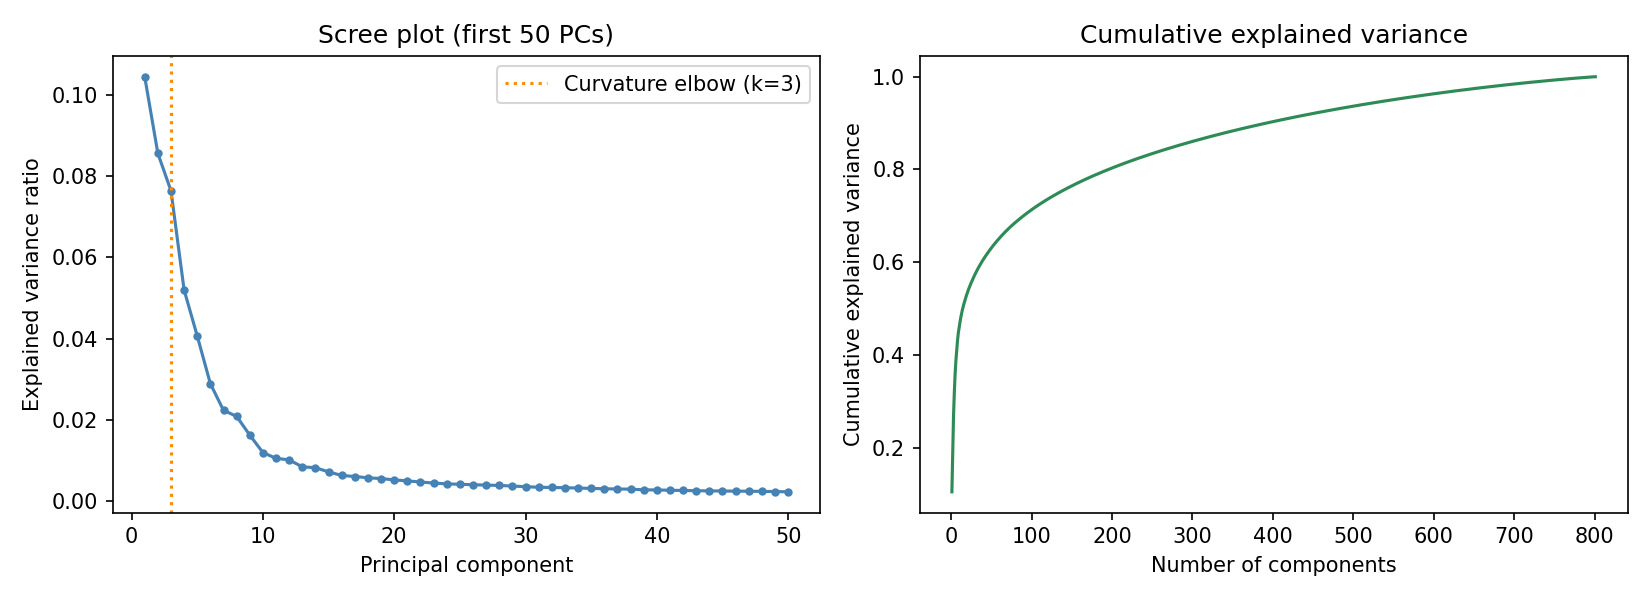
\includegraphics[width=0.95\textwidth]{../figures/scree_plot.png}
\caption{Scree plot of the real RNA-Seq covariance spectrum: per-component
explained variance (first 50 PCs, left) and cumulative explained variance
(all 801 components, right).}
\label{fig:scree}
\end{figure}

Figure~\ref{fig:corrdim} shows the log-log correlation integral for the
real data. The curve is smoothly convex across the full sampled radius
range with no long, sharply linear stretch; the automatically detected
scaling region (5 points, $r \in [149.6, 156.5]$) is narrow, reflecting
both the modest sample size ($N=801$) and the smoothly varying local
density typical of standardized, correlated gene-expression data, rather
than a sharply self-similar point cloud.

\begin{figure}[H]
\centering
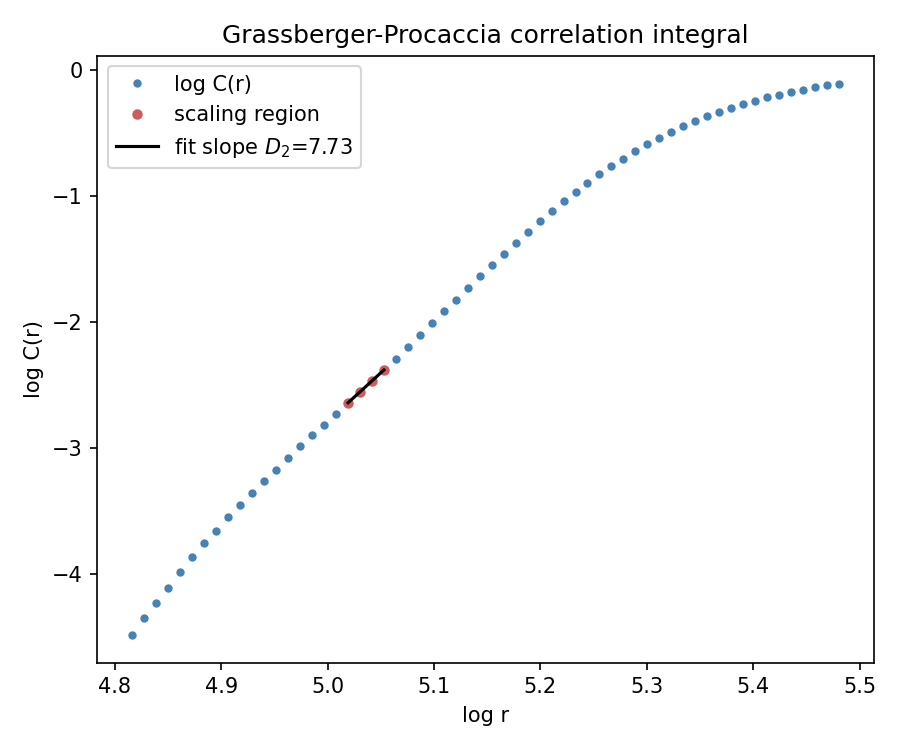
\includegraphics[width=0.7\textwidth]{../figures/log_log_correlation.png}
\caption{Log-log plot of the Grassberger--Procaccia correlation integral
$C(r)$ for the real RNA-Seq data, with the automatically detected scaling
region and fitted slope $D_2 = 7.73$ highlighted.}
\label{fig:corrdim}
\end{figure}

\section{Discussion: Reconciling the Three Estimators}
\label{sec:discussion}

The three estimators disagree substantially on the real data --
$D_2 \approx 7.7$, $k$-NN MLE mean $\approx 29.4$, Kaiser-criterion PCA
elbow at $100$, and $392$ components for $90\%$ linear variance -- and the
synthetic baselines show this disagreement is expected, not a symptom of
implementation error, since the same three estimators converge tightly on
the correct answer ($\approx 5$) for the linear manifold baseline once the
noise level is controlled (Table~\ref{tab:summary}).

$D_2$ and the $k$-NN MLE are both \emph{local} estimators: they infer
dimension from how the number of neighbors within a radius (or the ratio
of neighbor distances) scales, which directly reflects the manifold's
local geometry but is sensitive to the sparsity of pairwise distances when
$n$ is small relative to $d$ -- consistent with the well-documented
negative bias of both estimators in small-sample, high-dimensional
regimes, and with $D_2 < $ $k$-NN-MLE-mean here, since $D_2$'s scaling
region sits at a coarser radius scale where fewer effective neighbor pairs
constrain the fit. PCA, in contrast, is a \emph{global, linear} estimator:
it counts every direction of non-negligible variance, so it conflates true
low-dimensional nonlinear manifold structure (which a linear method must
represent using many linear components) with genuine additional
biological variance (subtype heterogeneity within each of the five cancer
types) and technical/batch variance, all three of which correlation
dimension and $k$-NN MLE are comparatively insensitive to at the local
neighborhood scale. The gap between the Kaiser elbow ($100$) and the
$90\%$-variance threshold ($392$) illustrates a further, distinct effect:
raw variance thresholds are dominated by the aggregate mass of the long
eigenvalue tail even when individual tail eigenvalues are small, which is
exactly the mechanism the noise-level sensitivity analysis
(Table~\ref{tab:noise-sweep}) demonstrates directly.

Taken together, the real data's estimates place a defensible working range
for the intrinsic dimension of the Pan-Cancer expression manifold at
roughly one to two orders of magnitude below the ambient dimension
$d = 20{,}264$ (single digits to a few dozen by local estimators, low
hundreds by the more permissive Kaiser/global criterion) -- far closer to
the $5$-class label cardinality than to $d$, and consistent with the
hypothesis that gene co-expression collapses the effective degrees of
freedom of a tumor's transcriptomic profile substantially below the number
of measured genes.

\section{Limitations}

The correlation dimension's automatically detected scaling region is
narrow (5 points) on the real data, so $D_2$ carries meaningful
finite-sample uncertainty not captured by the reported $R^2$ of the local
linear fit alone; a bootstrap over sample subsets would better
characterize this. The Kaiser and curvature elbow criteria are both
heuristics without a formal error rate; neither has a principled stopping
guarantee comparable to, e.g., a permutation-based significance test on
individual eigenvalues. The linear-manifold baseline validates recovery of
a \emph{linear} 5-dimensional ground truth; it does not test recovery of a
curved (nonlinear) low-dimensional manifold, which is the more realistic
model for biological data and is left to the nonlinear-embedding analysis
in Phase 3.

\section{References}

\begin{itemize}
\item Grassberger, P., \& Procaccia, I. (1983). Measuring the strangeness
of strange attractors. \emph{Physica D}, 9(1-2), 189--208.
\item Levina, E., \& Bickel, P. J. (2004). Maximum likelihood estimation
of intrinsic dimension. \emph{Advances in Neural Information Processing
Systems}, 17.
\item Weinstein, J. N., et al. (2013). The Cancer Genome Atlas Pan-Cancer
analysis project. \emph{Nature Genetics}, 45(10), 1113--1120.
\item Dataset: Gene Expression Cancer RNA-Seq (TCGA Pan-Cancer HiSeq),
\url{https://www.kaggle.com/datasets/debatreyadas/gene-expression-cancer-rna-seq}.
\end{itemize}

\appendix
\section{Appendix A: AI Usage Log}
See \texttt{ai\_usage\_log.md} in the repository root for the full,
incrementally maintained log. A Phase 2 entry documenting all
AI-generated modules, representative prompts, and verification steps for
this phase is included there.

\end{document}
